\chapter{General Introduction}

\section{The ocean, phytoplankton and why it matters}
"Phytoplankton is important. Phytoplankton is diverse. I want to look at phytoplankton diversity, particularly from a functional type point of view. Quantify diversity as it relates to ecosystem function (as production for example).

"it is amazing how little we actually know about phytoplankton globally and the effects that is has on biogeochemical cycles, and how it is affected by global change for example
"quite a few publications using models go too far in their extrapolations, whilst the general discussion still strongly revolves around meaningful model structures.. but no consensus is anywhere to be seen!
"need to identify the basic uncertainties and see if there is a way to discuss them scientifically
"Michaelis Menten kinetics are really outdated.. and i suppose using them in a trait-based modelling approach is questionable just the same
"plankton ecosystems are typically highly aggregated, a single variable gives the response of an incredibly diverse assemblage of phytoplankton species (P. Franks, 2009)


\section{Characterizing phytoplankton}
How did Researchers start dealing with Phytoplankton?

Two approaches to isolate strains, or take bulk properties

Obviously bulk properties also have to be taken from specific depth

so this adds the problem of the complexity of the physical environment that is the ocean, with enormous volume, turbulunce/mixing, diffusion and absorbance

XXX

"Phytoplankton can be characterised by many morphological, physiological, behavioural and life history traits and trade-offs \citep{Litchman2008, Litchman2010}.

"Studies on the phytoplankton community composition and their response to the environmental gradients are not novel. Ramón Margalef was probably one of the first ecologist to give an important momentum to the topic.  \citep{Margalef1978} used observations of key traits, such as nutrient utilization and sinking rates, to support his well known concept called "Margalef's mandala". His classification of phytoplankton functional types (PFTs) at different nutrient and turbulent environmental conditions represents an excellent first example of how the trait-based notion can be applied to better understand phytoplankton community ecology, therefore setting up the stage for further developments in the field.


\subsection{Functional types vs. traits}

XXXX


XXXX

\subsection{The relationship between diversity and ecosystem function}

XXXX


\section{Modeling phytoplankton communities}
Going into the details is necessary to understand the whole picture

One tool of integration are mathematical models

"The study of phytoplankton community structure, also promoted by the work of \citet{Falkowski1998}, is therefore very relevant in marine ecology and is especially important for understanding how phytoplankton will respond to a changing climate and with which consequences.



\begin{figure}
\centering
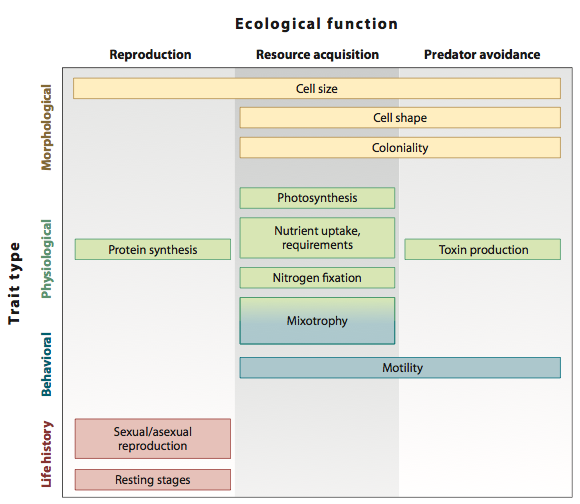
\includegraphics[width=0.7\linewidth]{./Chp1-Intro/Fig_litchman2008.png}
\caption[Scheme]{\small{Phytoplankton functional traits. Taken from \citet{Litchman2008}}}
\label{phytotrait}
\end{figure}

XXX

XXX

XXX

XXX. 

XXX

XXX

ALWAYS NEED A GOOD BASIS IN DATA TO VALIDATE MODELS AND HYPOTHESES

\section{The Cariaco basin \& the CARIACO time series}
XXXX

XXXX

XXX

THEN TALK ABOUT THE COLLAB/DATASHARE WITH JPINCKNEY AND CBENITEZNELSON, and how this allows an even deeper look at the biomass dynamics


\section{Aims of the proposed PhD project}
"The general goal of my Ph.D. project is to study the processes that structure the phytoplankton community in contrasting environmental regions of the Atlantic Ocean, using a trait-based modelling perspective. The specific aims during the course of the project are to:

\begin{itemize}
\item MANUSCRIPT 1 "Understanding Shifts in CARIACO"
\item MANUSCRIPT 2 "technical paper" - Geoscientific Model development
\item MANUSCRIPT 3 "BDEF in CARIACO"
\end{itemize}
